\chapter*{Introduction}
\addcontentsline{toc}{chapter}{Introduction}
Numerical weather prediction (NWP) presents a dynamic area of research in geophysical fluid dynamics. With computer models continuing to provide longer range predictions \cite{Cullen2006a} questions arise as to the limit of predictability of NWP. Whilst the mathematical theory underlying NWP has been in place as early as the 1900s, predictions were limited by the capabilities of available technology \cite{Golding2004}. It is widely recognised that NWP models are often time-costly and memory intensive. Of course, this is not the only limitation with chaos theory and the assimilation of observed data to be considered equally \cite{Weisheimer}. The increasing impact of extreme weather events on the world population means there is a vested interest in improving the predictability of NWP.
\\
\linebreak
This report is concerned with developing a numerical model for the formation of weather fronts, termed as frontogenesis.
With no formal mathematical definition we follow a definition offered by Hoskins \cite{Hoskins1982}, where fronts are considered as regions that have length scales comparable to the height of the domain considered, whilst exhibiting large gradients in other variables in the cross direction. Frontogenesis has been studied extensively \cite{Yamazaki2017, Cullen2008, Rotunno1994,Nakamura1988,Nakamura1994}, naturally, as it is a significant feature large-scale atmosphere flow (of the order 1000 \ km) \cite{Cullen2006a}. Fronts are most canonically recognised from surface pressure diagrams in weather forecasts as seen in \cite{fig:surfacepressure}
\\
\linebreak
This process will be studied under the idealised theoretical model provided by the Semi-Geostrophic (SG) equations the governing equations which we develop in Chapter \ref{governingequations}. Frontogenesis occurs as a result of a baroclinic instability \cite{Hoskins1982}, introduced in this project in the form of a vertical shear similar to the seminal work studied by Eady \cite{Eady}. As discussed by Mike Cullen in \cite{Cullen2006a} SG theory provides a highly predictable, general system for the study of large-scale atmospheric flow. 
\\
\linebreak
Work by B. Hoskins expressed the SG equations in \textquoteleft geostrophic co-ordinates\textquoteright \ \cite{Hoskins1972}. This was subsequently developed by Shutts and Cullen \cite{Shutts1987}. In this framework the SG equations exhibit interesting geometrical properties, namely it was shown that solutions can be sought as those of an equivalent Monge-Amp\`{e}re type optimal transport problem \cite{Cullen2006a}. This reformulation is discussed in chapter \ref{Chapter3}.
\\
\linebreak
Our focus now shifts to the numerical solution of the theoretical model through optimal transport methods. Following an idea from Dr Cotter, a solution using an efficient Damped Newton Algorithm (DA) recently developed by M\`{e}rigot et al. \cite{Merigot2017, Merigot2017a, Kitagawa2016} is explored. In Chapter \ref{OptimalTransport} we highlight the suitability of DA in solving the SG/EM equations for frontogenesis, and subsequently discuss how its implementation in building a numerical model for solving the semi-geostrophic equations is achieved in Chapter \ref{algorithm}.
\\
\linebreak
Finally, in Chapter \ref{results} we aim to validate the suitability of this numerical algorithm in solving the semi-geostrophic equations. This will be done through suitable analysis of the error as well as a qualitative comparison to results produced by other numerical models under similar conditions \cite{Nakamura1994,Cullen1993}.
\begin{figure}[h]
	\centering
	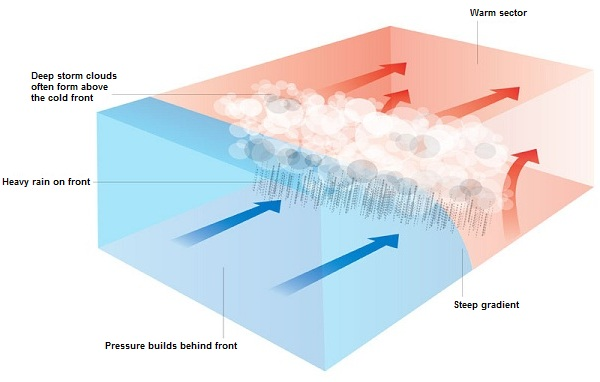
\includegraphics[width=0.5\linewidth]{introduction/figure-8-cold-front(image)}
	\caption[Cold Front]{The mechanism behind observed cold fronts as explained by the Met Office \cite{MetOffice2018}}
	\label{fig:figure-8-cold-frontimage}
\end{figure}
\begin{figure}[h]
	\centering
	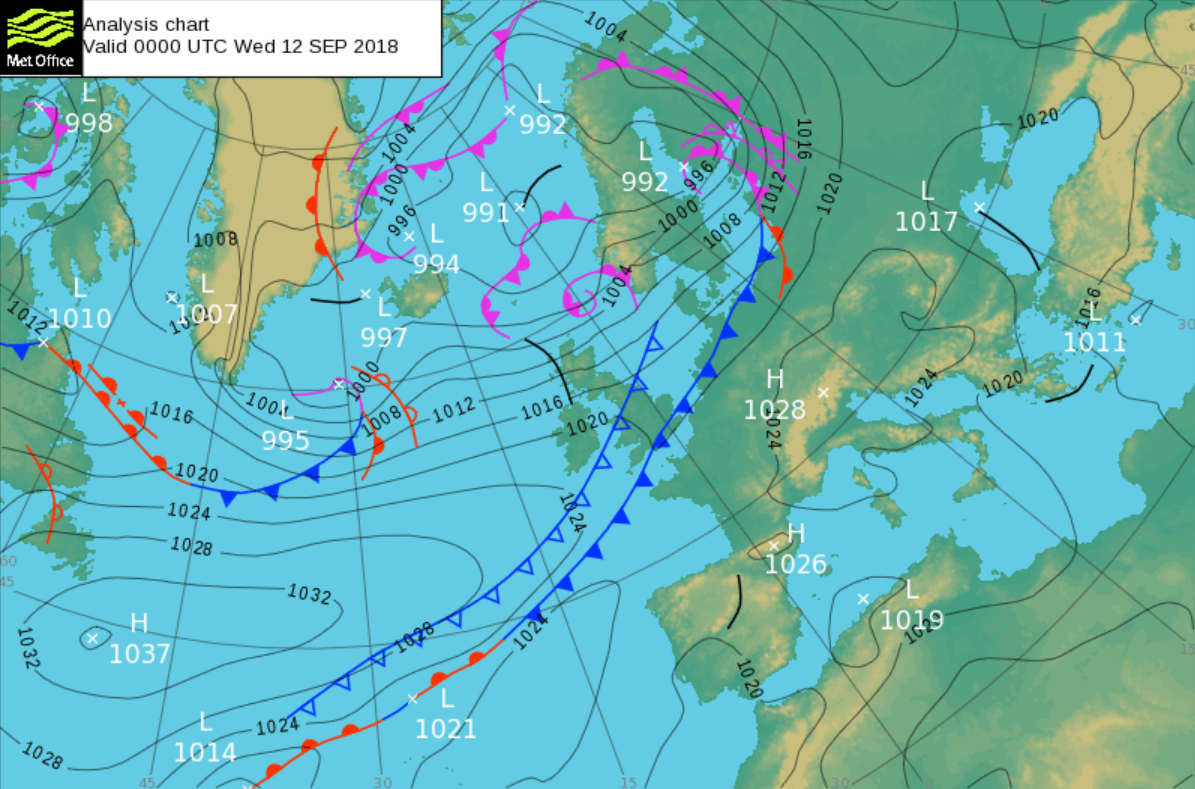
\includegraphics[width=0.5\linewidth]{introduction/surface_pressure}
	\caption[Surface Pressure Chart from 12/09/2018]{Surface Pressure Chart from 12/09/2018 from the Met Office website \cite{MetOffice2018a}}
	\label{fig:surfacepressure}
\end{figure}
